% !TEX program = XeLaTeX
\documentclass{VUMIFPSkursinis}
    \usepackage{algorithmicx}
    \usepackage{algorithm}
    \usepackage{algpseudocode}
    \usepackage{amsfonts}
    \usepackage{amsmath}
    \usepackage{bm}
    \usepackage{caption}
    \usepackage{color}
    \usepackage{enumitem}
    \usepackage{float}
    \usepackage{graphicx}
    \usepackage{listings}
    \usepackage{subfig}
    \usepackage{wrapfig}
    \usepackage{booktabs}
    \usepackage{blindtext}
    \usepackage{colortbl}
    \usepackage{graphicx}
    \usepackage{multirow}
    \usepackage{scrextend}
    \usepackage{longtable}
    \usepackage{enumitem}
    \usepackage{xparse}
    %\usepackage{tabularx}
    \usepackage{ltxtable}
    \usepackage{tabu}
    \usepackage{xcolor}
    % Titulinio aprašas
    \university{Vilniaus universitetas}
    \faculty{Matematikos ir informatikos fakultetas}
    \department{Programų sistemų katedra}
    \papertype{Laboratorinis darbas}
    \title{Skrydžių bilietų paieškos sistema}
    \titleineng{Plane tickets search system}
    \status{2 kurso 4 grupės studentai}
    \author{Olga Joana Šmitaitė}
    \secondauthor{Martynas Talalas}
    \thirdauthor{Nikita Gedgaudas}
    \fourthauthor{Justas Lakštinis}
    \date{Vilnius – \the\year}
    
    % Nustatymai
    % \setmainfont{Palemonas}   % Pakeisti teksto šriftą į Palemonas (turi būti įdiegtas sistemoje)
    \bibliography{bibliografija}
    
    \begin{document}
    \maketitle
      
        \tableofcontents
      
        \sectionnonum{Įvadas}
             Šis dokumentas papildo pirmąjį „Skrydžių bilietų paieškos sistemos“ dokumentą. Antroje versijoje yra atliekama robastiškumo analizė, preliminari projekto peržiūra ir apibrežiama techninė sistemos architektūra. Kaip ir pirmojoje dokumento versijoje, dokumente nurodomi sistemos reikalavimai, Statinė programų sistemos struktūra, užduotys ir, papildomai prisideda, techninė analizė. Reikalavimai išskirstyti į funkcinius ir nefunkcinius. Funkciniai reikalavimai nurodo pagrindines sistemos funkcijas, o nefunkciniai - nurodo kaip tas funkcijas sistema turi atlikti. Struktūrinės dalykinės srities modelis yra pateikiamas UML klasių diagramomis kartu su žodynais - sąrašu esybių su jų aprašymais. Užduočių skyrius aprašo sistemos atliekamas užduotis ir pasitelkus robastiškumo diagramomis parodyta kaip ir kokios sistemos dalys jas atliks. Techninės analizės skyriuje yra analizuojami techniniai sistemos aspektai - sistemos komponentai ir sistemos diegimas.
 
        \section{Reikalavimai}
			Šiame skyriuje išvardyti programų sistemos funkciniai ir nefunkciniai reikalavimai.
            \subsection{Funkciniai reikalavimai}
                \begin{enumerate}[label=\textbf{FR\arabic*}.]
                	\subsubsection{Bendri sistemos funkciniai reikalavimai}
                		\item \label{viena_puse} Sistema turi atlikti skrydžių į vieną pusę paiešką pagal:
						\begin{itemize}
                    		\item išvykimo datos intervalą (nuo/iki),
                    		\item skrydžio kainos intervalą (nuo/iki),
                    		\item išvykimo ir atvykimo vietas,
                    	\end{itemize}
						\item Sistema turi atlikti skrydžių į dvi puses paiešką pagal:
                    	\begin{itemize}
                    		\item išvykimo ir atvykimo datų intervalus (nuo/iki),
                    		\item skrydžio kainos intervalą (nuo/iki),
                    		\item išvykimo ir atvykimo vietas,
                    	\end{itemize}
                    	\item Sistema turi turėti galimybę rūšiuoti ir/arba  filtruoti paieškos rezultatus.
                    	\begin{enumerate}[label*=\textbf{\arabic*}.]
                        	\item Sistema rūšiuoja skrydžius pagal:
                        	\begin{itemize}
                            	\item greičiausius,
                            	\item pigiausius,
                            	\item optimaliausius (žr. \ref{optimalus}).
                        	\end{itemize}
                        	\item Sistema filtruoja skrydžius pagal:
                        	\begin{itemize}
                            	\item aviakompanijas,
                            	\item persėdimų skaičių.
                        	\end{itemize}
                    	\end{enumerate}
                    	\item \label{skrydzio_info} Pasirinkus skrydį sistema turi parodyti detalią skrydžio informaciją, kurioje yra:
                    	\begin{itemize}
                    		\item skrydžio išvykimo ir atvykimo datos ir laikai,
                    		\item skrydžio išvykimo ir atvykimo šalys, miestai ir oro uosto trumpiniai,
							\item skrydžio trukmė,
							\item skrydžio kaina.
                    	\end{itemize}
                    	\item Sistemoje turi būti galimybė vartotojui įsigyti skrydžio(-ų) bilietą, nukreipiant jį į atitinkamą aviakompanijos puslapį.
                    	\item Sistema atitinkamame lange vartotojui turi parodyti būsimus skrydžius, į kuriuos jis įsigijo bilietus.
                	\subsubsection{Papildomi funkciniai reikalavimai}
                    	\item \label{datos_ivedimas} Vartotojui norint įvesti datą, sistema turi pateikti mažą kalendorių arba leisti vartotojui savarankiškai įvesti datą.
                    	\item Paieškos formoje nieko neįvedus arba įvedus netinkamai, sistema turi pateikti vartotojui pavyzdį, kaip turėtų būti suvesti duomenys.
                \end{enumerate}
            \subsection{Nefunkciniai reikalavimai}
                \begin{enumerate}[label=\textbf{NFR\arabic*}.]
                	\subsubsection{Bendri sistemos nefunkciniai reikalavimai}
                		\item \label{lokalizacija} Sistema turi būti lietuvių kalba.
                		\item Programų sistema turi būti susieta su palaikomų aviakompanijų bilietų pirkimo svetainėmis.
                		\item \label{avia_db} Programų sistema turi turėti prieigą prie aviakompanijų duomenų bazių, kuriose saugomi tvarkaraščiai, naudotojai, įvykiai ir užrašai.
                		\item Programų sistema negali pažeisti Europos Žmogaus teisių ir pagrindinių laisvių apsaugos konvencijos
                	\subsubsection{Sistemos palaikymo ir veikimo reikalavimai}                	
                    	\item \label{operacines_sistemos} Sistema turi palaikyti tas operacines sistemas, kurios palaiko:
                    	\begin{itemize}
                        	\item Mozilla Firefox (nuo 58 versijos)
                        	\item Google Chrome (nuo 64 versijos)
                        	\item Microsoft Internet Explorer (nuo 11 versijos)
                        	\item Microsoft Edge (nuo 41 versijos)
                       	 	\item Apple Safari (nuo 11 versijos)
                    	\end{itemize}
                    	\item Sistema turi palaikyti HTTPS standartą.
                    	\item Programų sistemos palaikymui yra būtina bent 426 x 240 (240p 16:9) ekrano rezoliucija ir ekrano dydis turi būti bent 4‘‘.
                    	\item Įvykus sistemos sutrikimui, vartotojo darbo funkcionalumas turi būti atkurtas penkių minučių laikotarpyje.
                   	 	\item Didžiausia leistina programų sistemos apkrova yra 5000 vartotojų, prisijungusių vienu metu.
                    	\item Paieškos rezultatai pateikiami ne lėčiau kaip per 20 sekundžių.
                    	\item Programa turi būti įdiegta ir paleista serveryje, kuris veikia visomis metų dienomis 24 valandas per parą.
                    	\item Sisteminės klaidos turi būti išsaugojamos klaidų žurnale, kuris turi būti tikrinamas bent kartą per vieną darbo dieną
                    	\item Praplėtus programų sistemos funkcionalumą būtina patikrinti atnaujinimus prieš leidžiant jais naudotis vartotojams
					\subsubsection{Reikšmių reikalavimai}
                    	\item Datos įvedamos ir vaizduojamos DD/MM/YYYY formatu.
                    	\item Išvykimo data turi būti anksčiau arba sutapti su atvykimo data.
                    	\item Skrydžio kainos turi būti teigiamos ir rodomos eurais.
                    	\item Mažiausia skrydžio kaina turi būti mažesnė už didžiausią skrydžio kainą.
                    	\item Išvykimo ir atvykimo vietos negali sutapti.
                    	\item Vieta vaizduojama arba vedama formatu „<miestas> <oro uosto trijų raidžių trumpinys> <(nebūtina), šalis>“.
                    	\item \label{optimalus} Optimalesnis skrydis yra tas kurio kainos ir skrydžio trukmės santykis yra mažesnis.
                \end{enumerate}
      
        \section{Statinė programų sistemos struktūra}
            Šiame skyriuje pateikiamas struktūrinis nagrinėjamos dalykinės srities modelis. Modelis pateikiamas UML klasių diagramomis kartu su žodynu (žr. skyrius „Klasių diagrama“) - sąrašu esybių su jų aprašymais. Skyriaus pabaigoje pateikiama reikalavimų - struktūrinio dalykinės srities modelio atsekamumo matrica (žr. skyrius „Reikalavimų - struktūrinio dalykinės srities modelio atsekamumo matrica“).
            \subsection{Klasių diagrama}
            Čia pateikiama ir aprašoma sistemos klasių diagrama ir pateikiamas jos žodynas
                \begin{figure}[H]
                    \centering
                    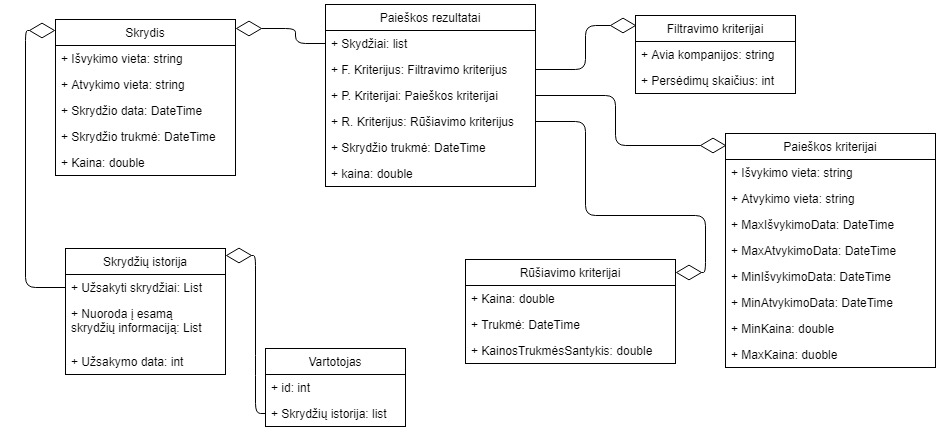
\includegraphics[scale=0.5]{img/class_diagram}
                    \caption{Klasių diagrama}
                    \label{klasių diagrama}
                \end{figure}
                \begin{enumerate}[label=\textbf{E\arabic*}.]
                    \item Paieškos rezultatai - aprašo skrydžių paieškos rezultatus pritaikius paieškos kriterijus.
                    \item Skrydis - detaliai aprašo skrydžio informaciją. Skrydžio informacija susideda iš išvykimo vietos, atvykimo vietos, skrydžio datos, skrydžio trukmės ir kainos.
                    \item Skrydžių istorija - aprašo vartotojo užsakytų, įvykusių bei būsimų skrydžių informaciją.
                    \item Filtravimo kriterijai - aprašo vartotojo nustatytus filtravimo kriterijus. Vartotojas gali pasirinkti norimas avia kompanijas ir pageidaujamų persėdimų skaičių
                    \item Paieškos kriterijai - aprašo vartotojo pasirinktus skrydžio bilietų paieškos kriterijus. Vartotojas gali nustatyti išvykimo vietą, atvikimo vietą, maksimalią ir minimalią išvykimo bei atvykimo datą, maksimalią bei minimalią kainą.
                    \item Rūšiavimo kriterijai - aprašo vartotojo pasirinktus skrydžių rūšiavimo kriterijus. Kriterijus sudaro kaina, skrydžio trukmė bei kainos ir trukmės santykis(optimalumas).
                    \item Vartotojas - asmuo naviguojantis skrydžių paieškos platformoje ir ieškantis reikiamų skrydžių.
                \end{enumerate}
    
            \subsection{Reikalavimų - struktūrinio dalykinės srities modelio atsekamumo matrica}
            Šiame skyriuje yra pateikiama reikalavimų - struktūrinės dalykinės srities modelio atsekamumo matrica (žr. \ref{Reikalavimų - struktūrinio dalykinės srities modelio atsekamumo matrica} lentelę). Matricoje pavaizduotos dalykinės srities modelio esybės bei sistemos funkciniai reikalavimai. Reikalavimų - struktūrinio dalykinės srities modelio atsekamumo matrica padeda susieti dalykinės srities modelio esybes su sistemos funkciniais(arba ne funkciniais) reikalavimais.
            \begin{table}[H]\footnotesize
                \centering
                \caption{Reikalavimų - struktūrinio dalykinės srities modelio atsekamumo matrica}
                {
                    \begin{tabular}{|c|c|c|c|c|c|c|c|c| }
                    \hline
                          & FR1  & FR2 & FR3 & FR4 & FR5 & FR6 & FR7 & FR8 \\ 
                    \hline
                        E1 & X   & X   & X   & X   &     &     &     &      \\  
                    \hline
                        E2 & X   & X   & X   & X   & X   & X   &     &      \\ 
                    \hline
                        E3 &     &     &     &     &     & X   &     &      \\ 
                    \hline
                        E4 &     &     & X   &     &     &     &     &      \\ 
                    \hline
                        E5 & X   & X   &     &     &     &     & X   & X    \\ 
                    \hline
                        E6 &     &     & X   &     &     &     &     &      \\ 
                    \hline
                        E7 & X   & X   & X   & X   & X   & X   & X   & X    \\ 
                    \hline 
                    \end{tabular}
                }
                \label{Reikalavimų - struktūrinio dalykinės srities modelio atsekamumo matrica}
            \end{table}
      
        \section{Užduotys}
        Šiame skyriuje pateikiamos sistemos atliekamos užduotys. Visos sistemos atliekamos užduotys yra atvaizduojamos užduočių diagramoje (žr. \ref{Užduočių diagrama}pav.). Atvaizdavus užduotis užduočių diagramoje, kiekviena užduotis yra detaliai aprašoma. Prie užduoties aprašymo yra pateikiami ir alternatyvūs scenarijai. Užduotims aprašyti taip pat yra naudojami ir kuriamos sistemos eskizai, leidžiantys geriau suprasti ir įsivaizduoti sistemos atliekamas užduotis. Skyriaus pabaigoje yra pateikiama ir reikalavimų - užduočių atsekamumo matrica.
            \begin{figure}[H]
                \centering
                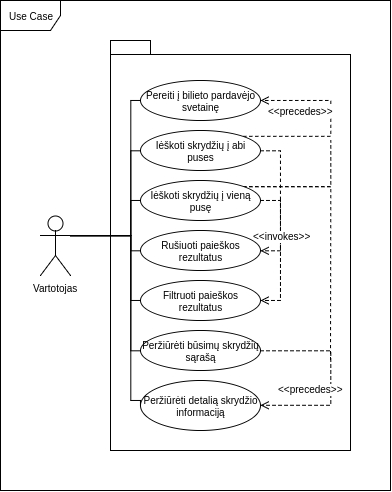
\includegraphics[scale=1]{img/use_case}
                \caption{Užduočių diagrama}
                \label{Užduočių diagrama}
            \end{figure}
            \subsection{Užduočių aprašymai}
                
                \begin{enumerate}[label=\textbf{U\arabic*}.]

                    \item \textbf{Ieškoti skrydžių į vieną pusę}\\
                    Vartotojas įveda išvykimo, atvykimo miestus. Pagal pageidavimą, įveda tinkamą išvykimo laiko intervalą, kainos intervalą. Tada vartotojas paspaudžia ant mygtuko „Ieškoti“ (žr. \ref{home_page_one_way}pav.) ir yra nukreipiamas į paieškos rezultatų langą, kur jam, lentelės pavidalu rodomi surasti skrydžiai pagal vartojojo įvestus kriterijus (žr. \ref{results_one_way} pav.).
                    \begin{figure}[H]
                        \centering
                        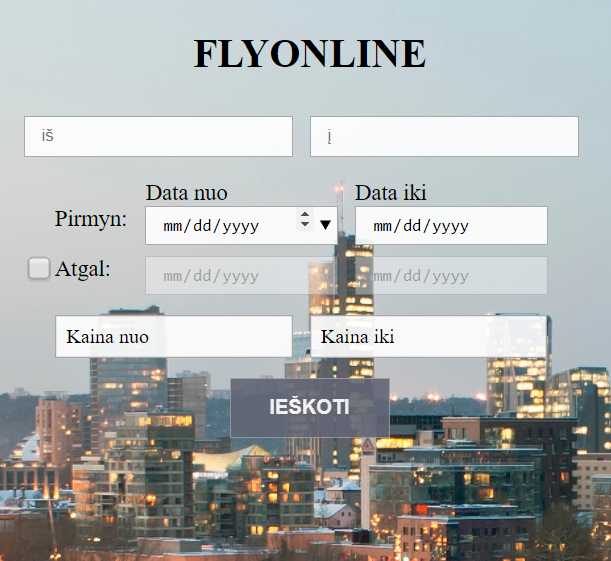
\includegraphics[scale=0.8]{img/oneway}
                        \caption{Pagrindinis puslapis}
                        \label{home_page_one_way}
                    \end{figure}
    
                    \begin{figure}[H]
                        \centering
                        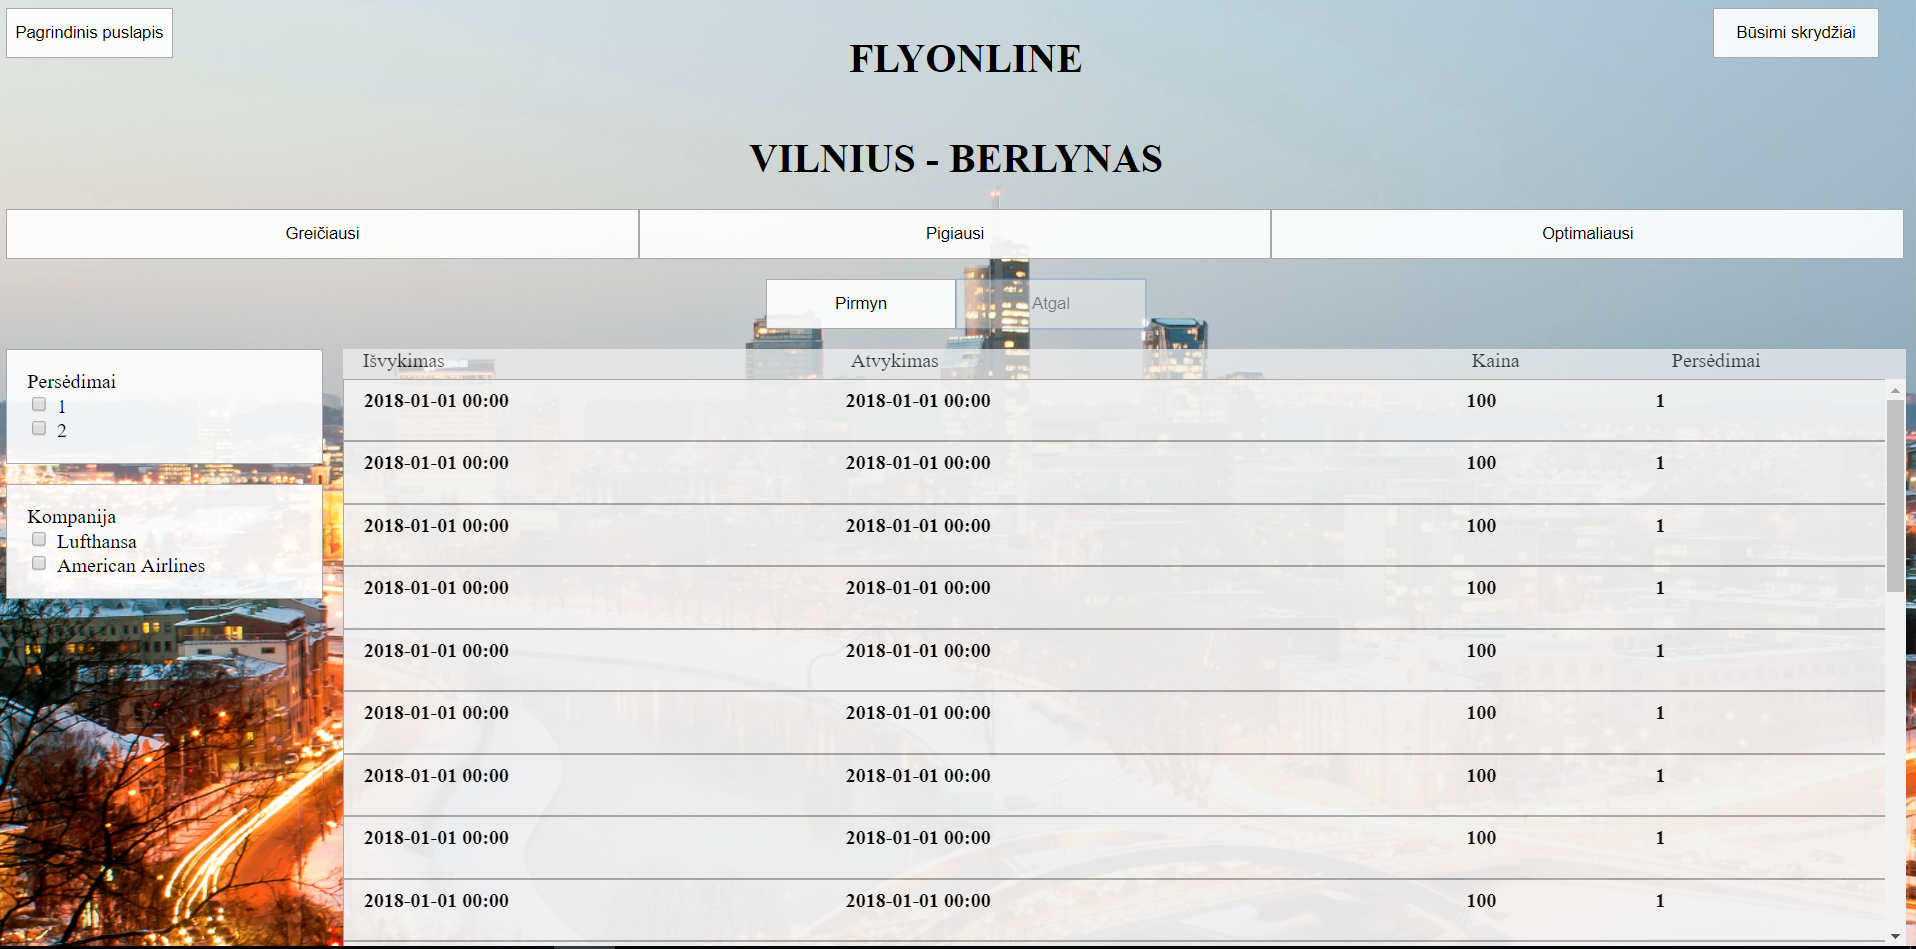
\includegraphics[scale=0.4]{img/search_one_way}
                        \caption{Paieškos rezultatai}
                        \label{results_one_way}
                    \end{figure}
                    \newpage\textbf{Alternatyvūs scenarijai:}
                    \begin{itemize}
                        \item Jei vartotojas neįveida atvykimo ir/ar išvykimo miestų, jam paspaudus ant mygtuko „Ieškoti“ jis nėra nukreipiamas į rezultatų langą. Išvykimo ar atvykimo miesto įvedimo laukas su neįvesta reikšme (arba abu), paženklinami raudonai.
                    \end{itemize}

                    \begin{figure}[H]
                        \centering
                        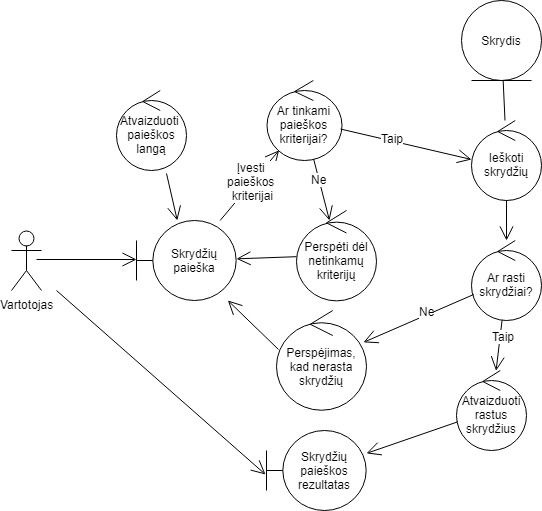
\includegraphics[scale=0.8]{img/ROBsearch}
                        \caption{Paieškos robastiškumo diagrama}
                        \label{home_page_one_way}
                    \end{figure}

                    \item \textbf{Ieškoti skrydžių į abi puses}\\
                    Vartotojas įveda išvykimo, atvykimo miestus. Pažymi varnele, kad renkasi skrydį atgal. Pagal pageidavimą, įveda išvykimo ir atvykimo tinkamų laikų intervalus, kainos intervalą. Tada vartotojas paspaudžia ant mygtuko „Ieškoti“ (žr. \ref{home_page_both_ways}pav.) ir yra nukreipiamas į paieškos rezultatų langą, kur jam, lentelės pavidalu rodomi surasti skrydžiai pagal vartojojo įvestus kriterijus (žr. \ref{results_both_ways} pav.).
                    \begin{figure}[H]
                        \centering
                        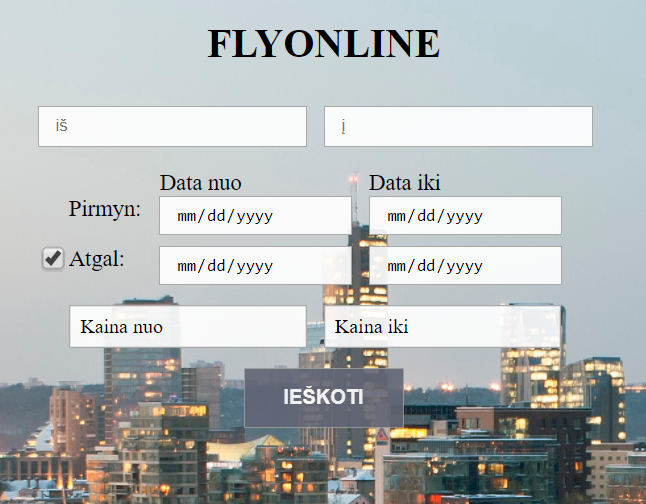
\includegraphics[scale=0.8]{img/bothways}
                        \caption{Pagrindinis puslapis}
                        \label{home_page_both_ways}
                    \end{figure}
    
                    \begin{figure}[H]
                        \centering
                        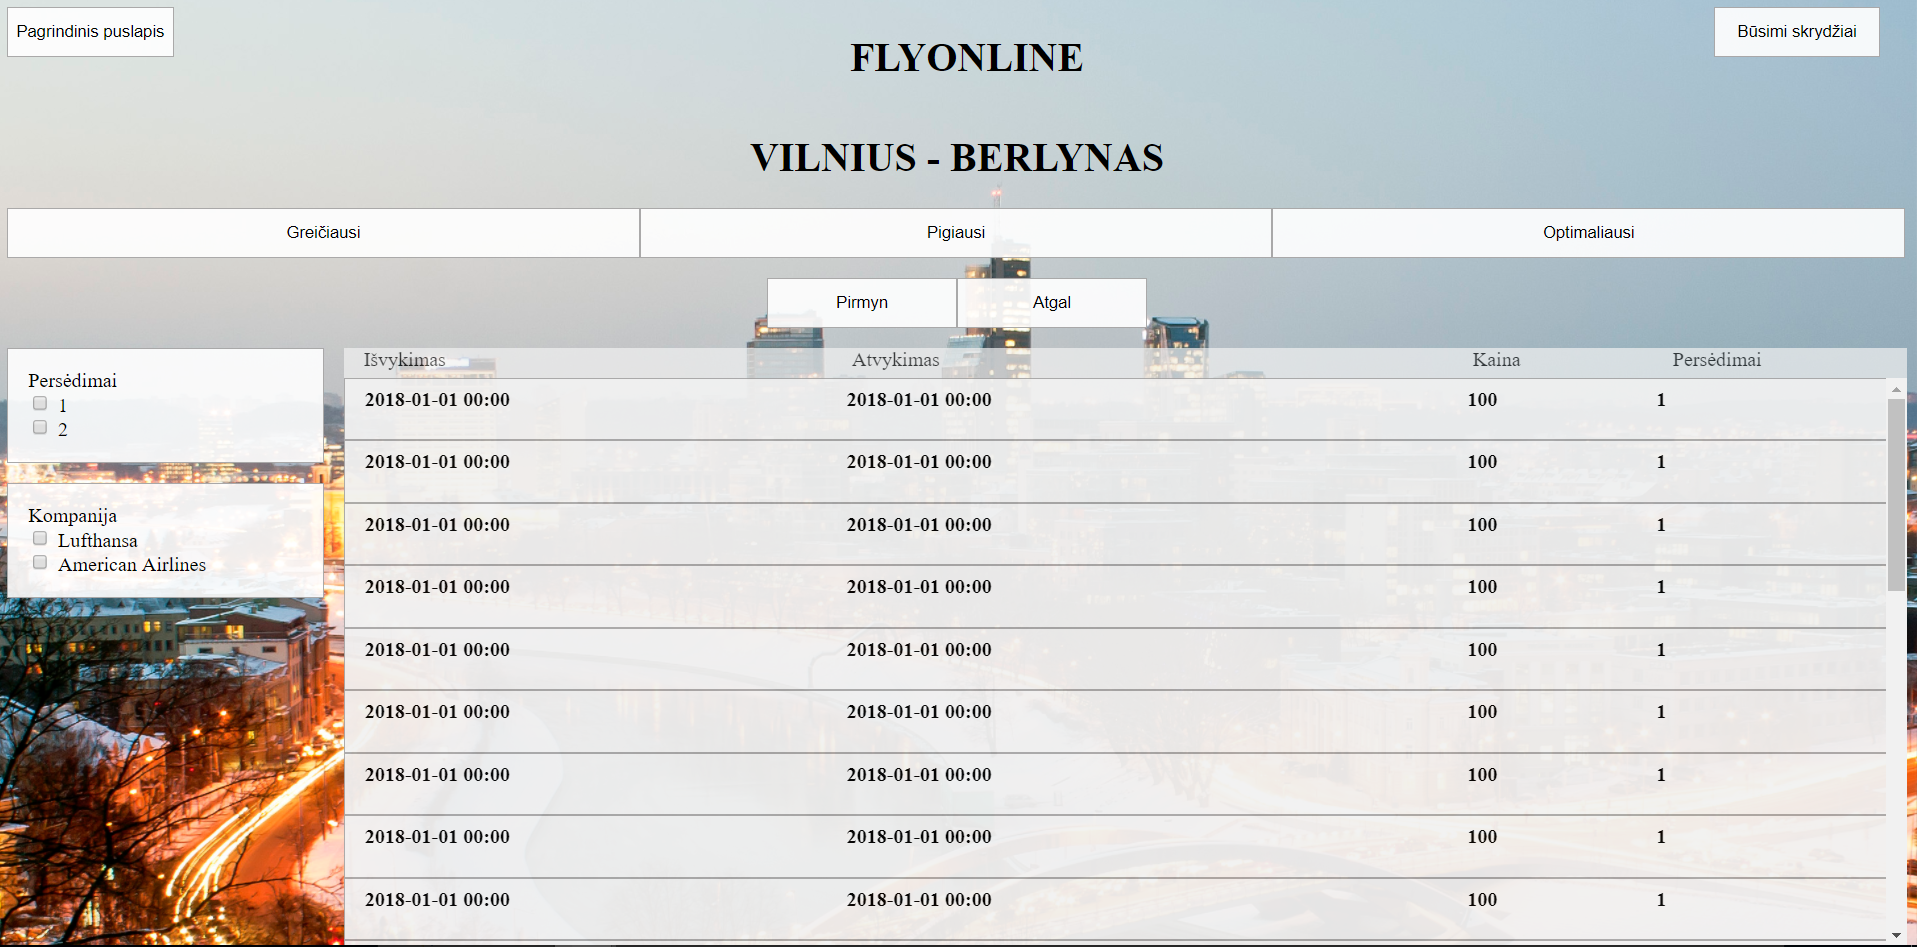
\includegraphics[scale=0.4]{img/search}
                        \caption{Paieškos rezultatai}
                        \label{results_both_ways}
                    \end{figure}
                    \textbf{Alternatyvūs scenarijai:}
                    \begin{itemize}
                        \item Jei vartotojas neįveida atvykimo ir/ar išvykimo miestų, jam paspaudus ant mygtuko „Ieškoti“ jis nėra nukreipiamas į rezultatų langą. Išvykimo ar atvykimo miesto įvedimo laukas su neįvesta reikšme (arba abu), paženklinami raudonai.
                    \end{itemize}

                    \item \textbf{Rušiuoti paieškos rezultatus}\\
                    Paieškos rezultatų lange, vartotojas pasirenka vieną iš trijų rūšiavimo būdus atitinkančių mygtukų: „Greičiausias“, „Pigiausias“ arba „Optimalus“ (žr. \ref{results_both_ways}pav., \ref{results_one_way} pav.). Paspaudus ant vieno iš jų, skrydžių paieškos rezultatai yra surūšiuojami pagal pasirinktą rušiavimo būdą.
                    \\\textbf{Alternatyvūs scenarijai:}
                    \begin{itemize}
                        \item Surušiavus rezultatus tam tikru pasirinktu būdu, vartotojas paspaudžia ant jau pasirinktą rūšiavimo būdą atitinkančio mygtuko. Rezultatai lieka surūšiuoti taip pat kaip ir prieš spaudžiant. 
                    \end{itemize}

                    \begin{figure}[H]
                        \centering
                        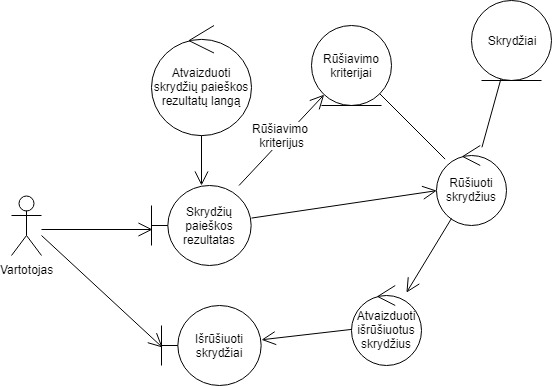
\includegraphics[scale=0.8]{img/ROBsort}
                        \caption{Rušiavimo robastiškumo diagrama}
                        \label{home_page_one_way}
                    \end{figure}

                    \item \textbf{Filtruoti paieškos rezultatus}\\
                    Paieškos rezultatų lange, vartotojas pažymi jį dominantį persėdimų skaičių ir skrydžių bendrovę (žr. \ref{results_both_ways}pav., \ref{results_one_way}pav.). Vartotojui pažymėjus konkrečią reikšmę ar to, ar ano, paieškos rezultatai yra iš karto atnaujinami, vaizduojant tik tuos skrydžius, kurie tenkina filtrų reikšmes.
                    \\\textbf{Alternatyvūs scenarijai:}
                    \begin{itemize}
                        \item Vartotojui pakartotinai paspaudus ant jau prieš tai pažymėta filtro reikšmės, rezultatai iš karto atsinaujina, o konkretus pažymėtas filtras nuimamas. Kai visi filtrai yra nuimti, rezultatai atsivaizduoja netaikant jiems jokio filtravimo.
                    \end{itemize}

                    \begin{figure}[H]
                        \centering
                        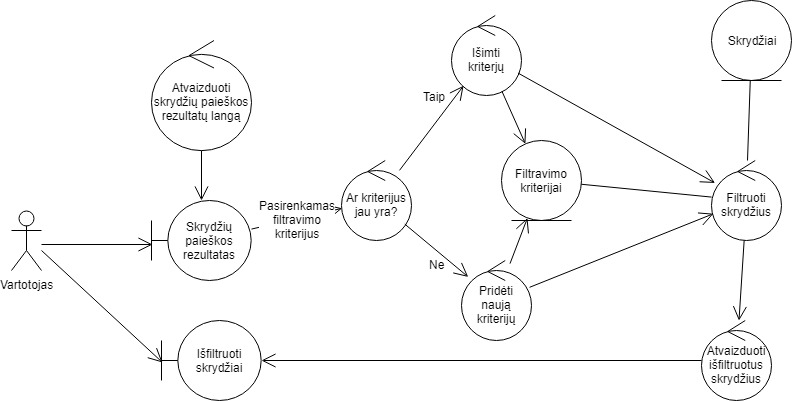
\includegraphics[scale=0.6]{img/ROBfilter}
                        \caption{Filtravimo robastiškumo diagrama}
                        \label{home_page_one_way}
                    \end{figure}

                    \item \textbf{Peržiūrėti detalią paieškos rezultato informaciją}\\
                    Vartotojas atlieka skrydžių paiešką. Spaudžia ant pasirinkto skrydžio iš sąrašo ir yra atidaromas dialogas su detlia skrydžio informacija (žr. \ref{search_result_details}pav.).
                    \begin{figure}[H]
                        \centering
                        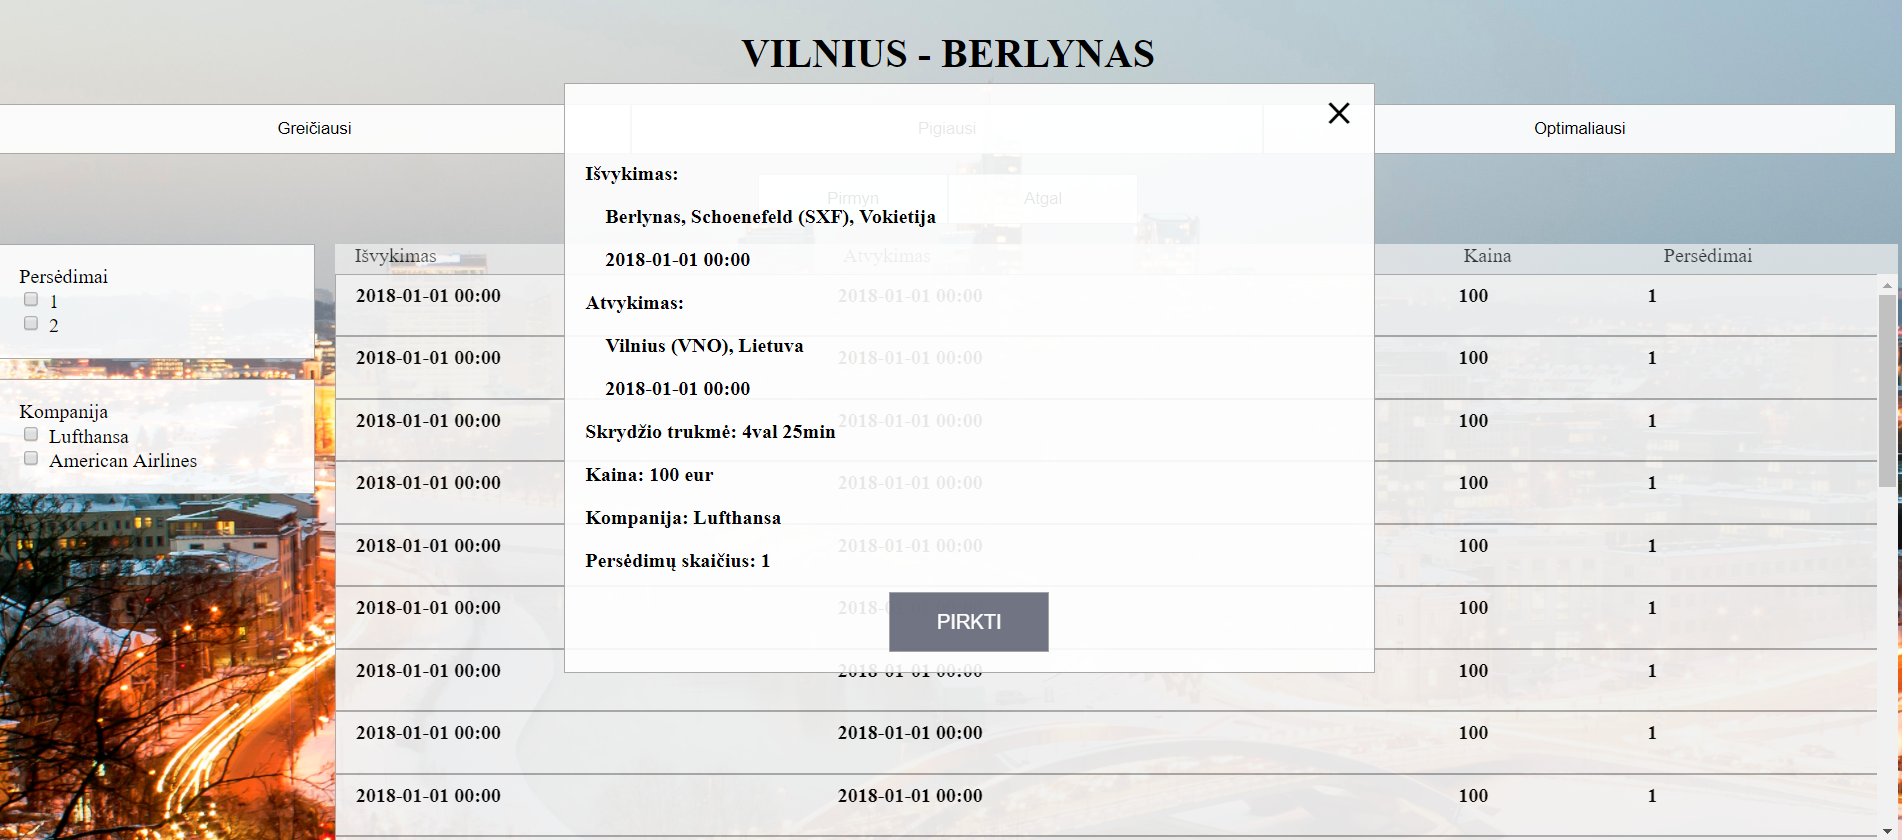
\includegraphics[scale=0.4]{img/buy}
                        \caption{Paieškos rezultato detalės}
                        \label{search_result_details}
                    \end{figure}

                    \begin{figure}[H]
                        \centering
                        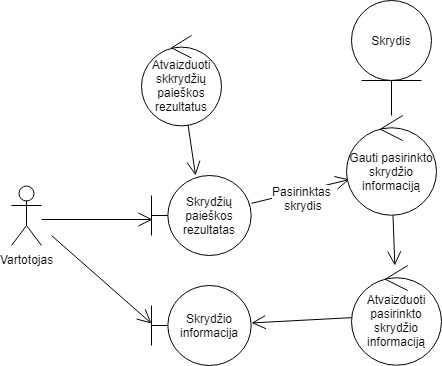
\includegraphics[scale=0.8]{img/ROBflight-info}
                        \caption{Detalios skrydžio informacijos peržiūros robastiškumo diagrama}
                        \label{home_page_one_way}
                    \end{figure}

                    \item \textbf{Pereiti į bilieto pardavėjo svetainę}\\
                    Vartotojas atlieka skrydžių paiešką. Spaudžia ant pasirinkto skrydžio. Atsidariusiame dialoge spaudžia mygtuką „Pirkti“ (žr. \ref{search_result_details}pav.) ir yra nukeliamas į bilieto pardavėjo puslap.


                    \begin{figure}[H]
                        \centering
                        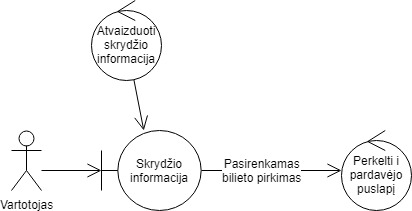
\includegraphics[scale=0.8]{img/ROBbuy}
                        \caption{Perėjimo i bilietu pardavėjo svetainę robastiškumo diagrama}
                        \label{home_page_one_way}
                    \end{figure}

                    \item \textbf{Peržiūrėti būsimų skrydžių sąrašą}\\
                    Vartotojas spaudžia ant mygtuko „Būsimi skrydžiai“. Atidaromas skrydžių, į kuriuos vartotojas yra įsigijęs bilietus sąrašas (žr. \ref{upcoming}pav.).
                    \begin{figure}[H]	
                        \centering
                        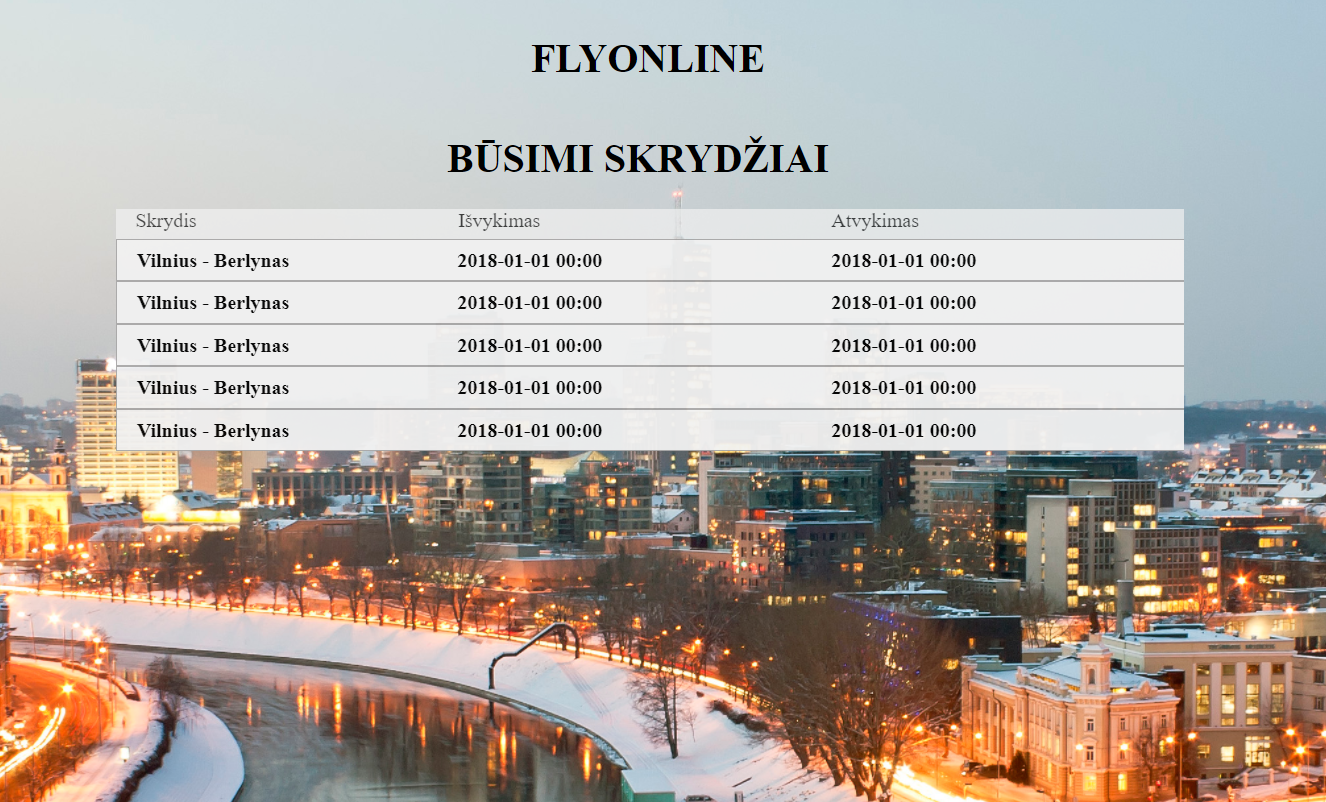
\includegraphics[scale=0.6]{img/history}	
                        \caption{Būsimų skrydžių sąrašas}	
                        \label{upcoming}	
                    \end{figure}
                    \newpage\textbf{Alternatyvūs scenarijai:}
                    \begin{itemize}
                        \item Jei būsimų skrydžių sąrašas yra tuščias, sąrašo vietoje vartotojui parodoma žinutė „Sąrašas yra tuščias“.
                    \end{itemize}

                    \begin{figure}[H]
                        \centering
                        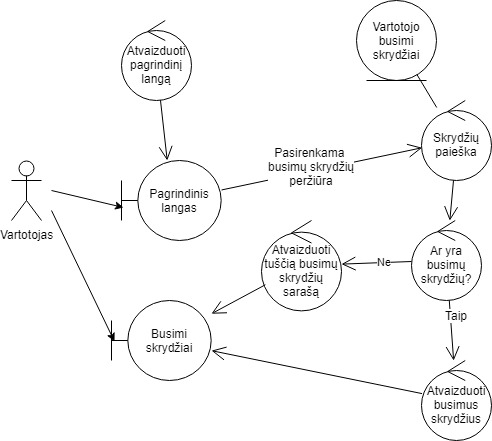
\includegraphics[scale=0.8]{img/ROBflights}
                        \caption{Būsimų skrydžių peržiūros robastiškumo diagrama}
                        \label{home_page_one_way}
                    \end{figure}

                    \item \textbf{Peržiūrėti detalią būsimo skrydžio informaciją}\\
                    Vartotojas atidaro būsimų skrydžių sąraša. Spaudžia ant pasirinkto skrydžio iš sąrašo ir yra atidaromas dialogas su išsamia skrydžio informacija (žr. \ref{upcoming_fligth_details}pav.).
                    \begin{figure}[H]	
                        \centering
                        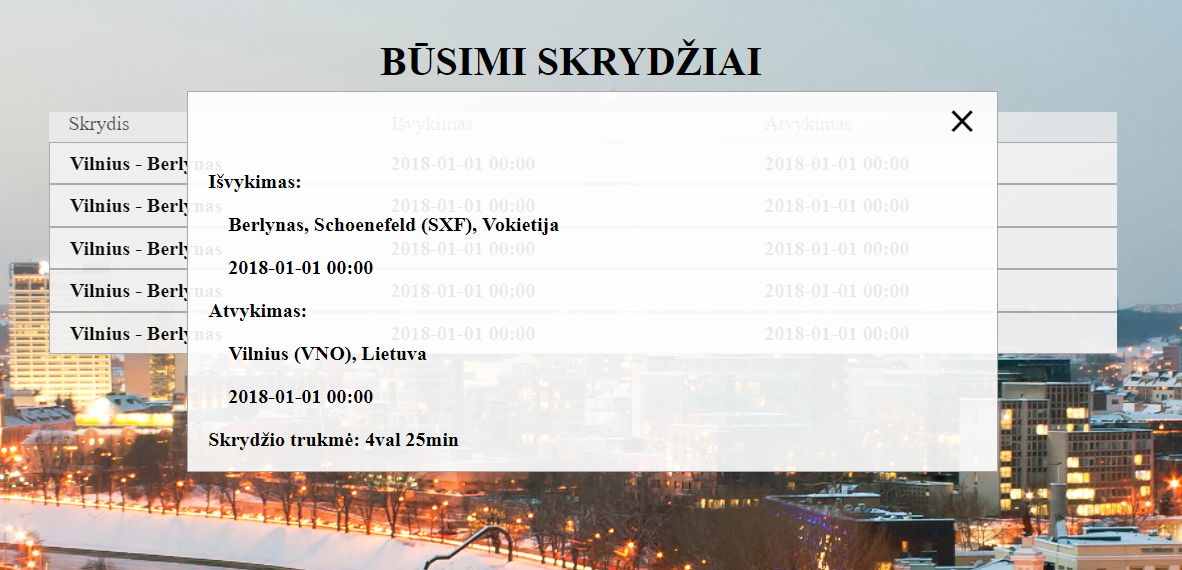
\includegraphics[scale=0.6]{img/details}	
                        \caption{Būsimo skrydžio informacija}	
                        \label{upcoming_fligth_details}	
                    \end{figure}

                    \begin{figure}[H]
                        \centering
                        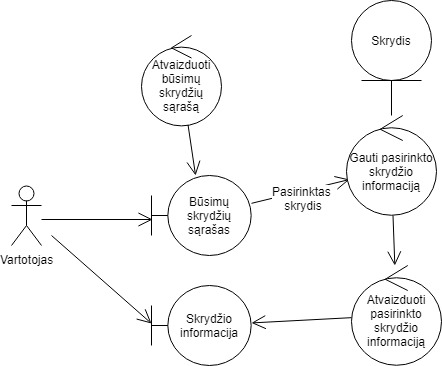
\includegraphics[scale=0.8]{img/ROBupcoming-flight-info}
                        \caption{Detalios būsimo skrydžio informacijos robastiškumo diagrama}
                        \label{home_page_one_way}
                    \end{figure}
                    
                \end{enumerate}
      
            \subsection{Reikalavimų - užduočių atsekamumo matrica}
            Šiame poskyryje pateikiama reikalavimų - užduočių atsekamumo matrica. Matricoje pavaizduotos užduotys(Use cases) bei reikalavimai. Ši matrica padeda atsekti kurios užduotys įgyvendina atitinkamus reikalavimus (žr. \ref{matrix2}pav.).
            \begin{table}[H]\footnotesize
                \centering
                \caption{Reikalavimų - užduočių atsekamumo matrica}
                \label{matrix2}
                {
                    \begin{tabular}{|c|c|c|c|c|c|c|c|c| }
                    \hline
                        & FR1 & FR2 & FR3 & FR4 & FR5 & FR6 & FR7 & FR8 \\ 
                    \hline
                     U1 & X   &     &     &     &     &     & X   & X    \\ 
                    \hline
                     U2 &     & X   &     &     &     &     & X   & X    \\  
                    \hline
                     U3 &     &     & X   &     &     &     &     &      \\ 
                    \hline
                     U4 &     &     & X   &     &     &     &     &      \\ 
                    \hline
                     U5 &     &     &     & X   &     &     &     &      \\ 
                    \hline
                     U6 &     &     &     &     & X   &     &     &      \\ 
                    \hline
                     U7 &     &     &     &     &     & X   &     &      \\ 
                    \hline
                     U8 &     &     &     & X   &     &     &     &      \\ 
                    \hline 
                    \end{tabular}
                }
            \end{table}
    \section{Techninė analizė}
      Šis skyrius aprašo siūlomą techinė architektūrą, sukurtą atsižvelgiant į pastabas, iškeltas atliekant robastiškumo analizę bei preliminarią projekto peržiūrą.
      \subsection{Komponentinė sandara}
      Čia pateikiama sistemos komponentinė sandara ir jos aprašymas
        \begin{figure}[H]
          \centering
          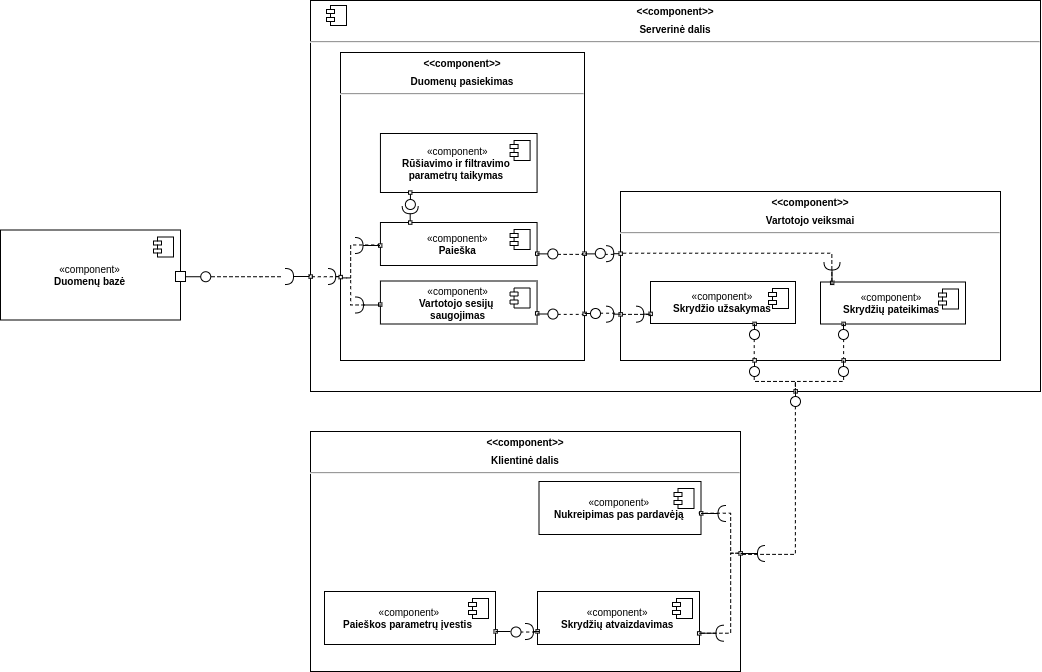
\includegraphics[scale=0.45]{img/Komponentai}
          \caption{Sistemos komponentinė sandara (UML Komponentų diagrama)}
          \label{components}
        \end{figure}
        Visą sistemą galima suskaidyti į tris pagrindinius komponentus: Klientinę dalį, Serverinę dalį bei Duomenų bazę (žr. \ref{components}pav.). Šių trijų komponentų rolės atitinka „3-tier“ architektūros sandarą - Atvaizdavimo sluoksnį, Verslo taisyklių sluoksnį bei Duomenų sluoksnį. Smulkesnis skaidymas į komponentus yra pagal funkcinius sistemos aspektus. Tai padaryta siekiant užtikrinti vykdomojo kodo testavimo ir bendrai palaikymo paprastumą, bei suteikia galimybę paprastesniam plečiamumui bei lankstensiam diegimui. 
      \subsection{Diegimas}
      Čia aprašomas sistemos diegimas
        \begin{figure}[H]
          \centering
          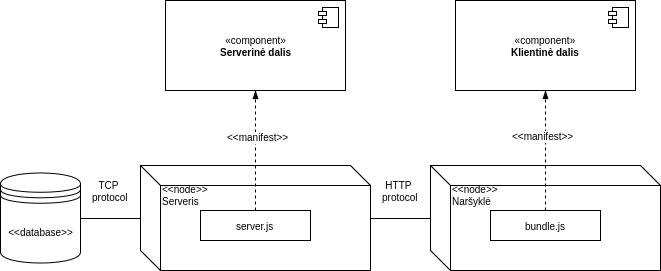
\includegraphics[scale=0.7]{img/Diegimas}
          \caption{Sistemos diegimas (UML Diegimo diagrama, UML Manifestacijos diagrama)}
          \label{deployment}
        \end{figure}
        Sistemos komponentų diegimas yra trivialus, pilnai dengiantis užsakovo dabartinius poreikius. Klasikinis kliento-serverio sistemos diegimas leidžia lengvai susieti įrangos kūrimo procesą su pastoviu atnaujinimų (Conitinuous Integration), be to, minimizuoja tikimybę sisteminių klaidų dėl tinklo ar diegimo kliūčių. Kylant poreikiui, šią sistemą lengva klasterizuoti, kas garantuoja stabilumą ir nebrangų palaikomumą (žr. \ref{deployment}pav.).
    \section{Testavimo planas ir scenarijai}
        \subsection{Skrydžių paieškos langas}
            \noindent\textbf{Reikalavimai testui:} Atidarytas skrydžių paieškos langas. \\

            \noindent\textbf{Scenarijus:}
                \begin{enumerate}
                    \item Vartotojas suveda skirtingus išvykimo ir atvykimo miestus.
                    \item Suveda būsimą kelionės pirmyn datos intervalą („Data nuo“ yra ankstesnė arba lygi „Datai iki“).
                    \item Spaudžia „Ieškoti“.
                \end{enumerate}
            \textbf{Rezultatas:} Atsidaro skrydžių paieškos rezultatų langas, kuriame rodomas paieškos kriterijus atitinkančių skrydžių į vieną pusę sąrašas.\\
            
            \noindent\textbf{Scenarijus:}
                \begin{enumerate}
                    \item Vartotojas pažymi „Atgal“.
                \end{enumerate}
            \textbf{Rezultatas:} Kelionės atgal datos intervalo įvedimo laukai tampa redaguojami.\\
            
            \noindent\textbf{Scenarijus:}
                \begin{enumerate}
                    \item Vartotojas suveda skirtingus išvykimo ir atvykimo miestus.
                    \item Suveda būsimą kelionės pirmyn datos intervalą („Data nuo“ yra ankstesnė arba lygi „Datai iki“).
                    \item Pažymi „Atgal“.
                    \item Suveda būsimą kelionės atgal datos intervalą („Data nuo“ yra ankstesnė arba lygi „Datai iki“).
                    \item Spaudžia „Ieškoti“.
                \end{enumerate}
            \textbf{Rezultatas:} Atsidaro skrydžių paieškos rezultatų langas, kuriame rodomas paieškos kriterijus atitinkančių skrydžių į abi puses sąrašas.\\
            
            \noindent\textbf{Scenarijus:}
                \begin{enumerate}
                    \item Vartotojas suveda vienodus išvykimo ir atvykimo miestus.
                    \item Suveda būsimą kelionės pirmyn datos intervalą („Data nuo“ yra ankstesnė arba lygi „Datai iki“).
                    \item Spaudžia „Ieškoti“.
                \end{enumerate}
            \textbf{Rezultatas:} Miestų įvedimo laukai paryškinami raudonai.\\
            
            \noindent\textbf{Scenarijus:}
                \begin{enumerate}
                    \item Vartotojas suveda išvykimo miestą.
                    \item Suveda būsimą kelionės pirmyn datos intervalą („Data nuo“ yra ankstesnė arba lygi „Datai iki“).
                    \item Spaudžia „Ieškoti“.
                \end{enumerate}
            \textbf{Rezultatas:} Atvykimo miesto įvedimo laukas paryškinamas raudonai.\\
            
            \noindent\textbf{Scenarijus:}
                \begin{enumerate}
                    \item Vartotojas suveda atvykimo miestą.
                    \item Suveda būsimą kelionės pirmyn datos intervalą („Data nuo“ yra ankstesnė arba lygi „Datai iki“).
                    \item Spaudžia „Ieškoti“.
                \end{enumerate}
            \textbf{Rezultatas:} Išvykimo miesto įvedimo laukas paryškinamas raudonai.\\
            
            \noindent\textbf{Scenarijus:}
                \begin{enumerate}
                    \item Vartotojas suveda būsimą kelionės pirmyn datos intervalą („Data nuo“ yra ankstesnė arba lygi „Datai iki“).
                    \item Spaudžia „Ieškoti“.
                \end{enumerate}
            \textbf{Rezultatas:} Miestų įvedimo laukai paryškinami raudonai.\\
            
            \noindent\textbf{Scenarijus:}
                \begin{enumerate}
                    \item Vartotojas suveda skirtingus išvykimo ir atvykimo miestus.
                    \item Suveda būsimą kelionės pirmyn datos intervalą („Data nuo“ yra vėlesnė už „Datą iki“).
                    \item Spaudžia „Ieškoti“.
                \end{enumerate}
            \textbf{Rezultatas:} Skrydžio pirmyn datos intervalo įvedimo laukai paryškinami raudonai.\\
            
            \noindent\textbf{Scenarijus:}
                \begin{enumerate}
                    \item Vartotojas suveda skirtingus išvykimo ir atvykimo miestus.
                    \item Spaudžia „Ieškoti“.
                \end{enumerate}
            \textbf{Rezultatas:} Skrydžio pirmyn datos intervalo įvedimo laukai paryškinami raudonai.\\
            
            \noindent\textbf{Scenarijus:}
                \begin{enumerate}
                    \item Vartotojas suveda skirtingus išvykimo ir atvykimo miestus.
                    \item Suveda būsimą kelionės pirmyn datos intervalą („Data nuo“ yra ankstesnė arba lygi „Datai iki“).
                    \item Pažymi „Atgal“.
                    \item Suveda būsimą kelionės atgal datos intervalą („Data nuo“ yra vėlesnė už „Datą iki“).
                    \item Spaudžia „Ieškoti“.
                \end{enumerate}
            \textbf{Rezultatas:} Skrydžio atgal datos intervalo įvedimo laukai paryškinami raudonai.\\
            
            \noindent\textbf{Scenarijus:}
                \begin{enumerate}
                    \item Vartotojas suveda skirtingus išvykimo ir atvykimo miestus.
                    \item Suveda būsimą kelionės pirmyn datos intervalą („Data nuo“ yra ankstesnė arba lygi „Datai iki“).
                    \item Pažymi „Atgal“.
                    \item Spaudžia „Ieškoti“.
                \end{enumerate}
            \textbf{Rezultatas:} Skrydžio atgal datos intervalo įvedimo laukai paryškinami raudonai.\\
            
        \subsection{Rezultatų filtravimas}
        \subsection{Rezultatų rūšiavimas}
        \subsection{Skrydžio informacijos peržiūra}
        \subsection{Nukreipimas į bilietų platintojo puslapį}
    \sectionnonum{Išvados ir rezultatai}
			Atlikus robastiškumo analizę, preliminarią projekto peržiūrą ir apibrežus techninę sistemos architektūrą (dalį ICONIX proceso žingsnių) pastebėjome, kad šioje darbo fazėje pirminiai sistemos reikalavimai atitinka sistemos numatomas užduotis, todėl programų sistemos reikalavimai nebuvo keisti.
			
		\sectionnonum{Pakeitimų sąrašas}
			\begin{enumerate}
				\item Skyrius „Struktūrinis dalykinės srities modelis“ perdarytas į „Statinė programų sistemos struktūra“,
				\item Apibrėžta techninė sistemos analizė,
				\item Užduočių aprašymuose pridėtos robastiškumo diagramos.
			\end{enumerate}
        \sectionnonum{Šaltiniai}
        Analizuojant kuriamą sistemą, kuriant sistemos reikalavimus, apibrėžiant struktūrinį dalykinės sryties modelį bei aprašant sistemos atliekamas užduotis buvo remtasi šia literatūra:
            \begin{enumerate}
                \item Don Rosenberg ir Matt Stephens. \textit{Use Case Driven Object Modeling with UML Theory and Practice}. Apress, 2007.
            \end{enumerate}
      
    \end{document}
      